\documentclass{article}
\usepackage{amsmath, amssymb, amsfonts}
\usepackage{natbib}
\usepackage{graphicx}
\usepackage{hyperref}
\usepackage{tikz}
\usetikzlibrary{bayesnet}
\usetikzlibrary{positioning}
\usepackage{algorithm}
\usepackage[noend]{algorithmic}
% ------------------------------------------------------------------------
% Packages
% ------------------------------------------------------------------------
\usepackage{amsmath}

% ------------------------------------------------------------------------
% Macros
% ------------------------------------------------------------------------
%~~~~~~~~~~~~~~~
% List shorthand
%~~~~~~~~~~~~~~~
\newcommand{\BIT}{\begin{itemize}}
\newcommand{\EIT}{\end{itemize}}
\newcommand{\BNUM}{\begin{enumerate}}
\newcommand{\ENUM}{\end{enumerate}}
%~~~~~~~~~~~~~~~
% Text with quads around it
%~~~~~~~~~~~~~~~
\newcommand{\qtext}[1]{\quad\text{#1}\quad}
%~~~~~~~~~~~~~~~
% Shorthand for math formatting
%~~~~~~~~~~~~~~~
\newcommand\mbb[1]{\mathbb{#1}}
\newcommand\mbf[1]{\mathbf{#1}}
\def\mc#1{\mathcal{#1}}
\def\mrm#1{\mathrm{#1}}
%~~~~~~~~~~~~~~~
% Common sets
%~~~~~~~~~~~~~~~
\def\reals{\mathbb{R}} % Real number symbol
\def\integers{\mathbb{Z}} % Integer symbol
\def\rationals{\mathbb{Q}} % Rational numbers
\def\naturals{\mathbb{N}} % Natural numbers
\def\complex{\mathbb{C}} % Complex numbers
\def\simplex{\mathcal{S}} % Simplex
%~~~~~~~~~~~~~~~
% Common functions
%~~~~~~~~~~~~~~~
\renewcommand{\exp}[1]{\operatorname{exp}\left(#1\right)} % Exponential
\def\indic#1{\mbb{I}\left({#1}\right)} % Indicator function
\providecommand{\argmax}{\mathop\mathrm{arg max}} % Defining math symbols
\providecommand{\argmin}{\mathop\mathrm{arg min}}
\providecommand{\arccos}{\mathop\mathrm{arccos}}
\providecommand{\asinh}{\mathop\mathrm{asinh}}
\providecommand{\dom}{\mathop\mathrm{dom}} % Domain
\providecommand{\range}{\mathop\mathrm{range}} % Range
\providecommand{\diag}{\mathop\mathrm{diag}}
\providecommand{\tr}{\mathop\mathrm{tr}}
\providecommand{\abs}{\mathop\mathrm{abs}}
\providecommand{\card}{\mathop\mathrm{card}}
\providecommand{\sign}{\mathop\mathrm{sign}}
\def\rank#1{\mathrm{rank}({#1})}
\def\supp#1{\mathrm{supp}({#1})}
%~~~~~~~~~~~~~~~
% Common probability symbols
%~~~~~~~~~~~~~~~
\def\E{\mathbb{E}} % Expectation symbol
\def\Earg#1{\E\left[{#1}\right]}
\def\Esubarg#1#2{\E_{#1}\left[{#2}\right]}
\def\P{\mathbb{P}} % Probability symbol
\def\Parg#1{\P\left({#1}\right)}
\def\Psubarg#1#2{\P_{#1}\left[{#2}\right]}
\def\Cov{\mrm{Cov}} % Covariance symbol
\def\Covarg#1{\Cov\left[{#1}\right]}
\def\Covsubarg#1#2{\Cov_{#1}\left[{#2}\right]}
\def\Var{\mrm{Var}}
\def\Vararg#1{\Var\left(#1\right)}
\def\Varsubarg#1#2{\Var_{#1}\left(#2\right)}
\newcommand{\family}{\mathcal{P}} % probability family
\newcommand{\eps}{\epsilon}
\def\absarg#1{\left|#1\right|}
\def\msarg#1{\left(#1\right)^{2}}
\def\logarg#1{\log\left(#1\right)}
%~~~~~~~~~~~~~~~
% Distributions
%~~~~~~~~~~~~~~~
\def\Gsn{\mathcal{N}}
\def\Ber{\textnormal{Ber}}
\def\Bin{\textnormal{Bin}}
\def\Unif{\textnormal{Unif}}
\def\Mult{\textnormal{Mult}}
\def\Cat{\textnormal{Cat}}
\def\Gam{\textnormal{Gam}}
\def\InvGam{\textnormal{InvGam}}
\def\NegMult{\textnormal{NegMult}}
\def\Dir{\textnormal{Dir}}
\def\Lap{\textnormal{Laplace}}
\def\Bet{\textnormal{Beta}}
\def\Poi{\textnormal{Poi}}
\def\HypGeo{\textnormal{HypGeo}}
\def\GEM{\textnormal{GEM}}
\def\BP{\textnormal{BP}}
\def\DP{\textnormal{DP}}
\def\BeP{\textnormal{BeP}}
%~~~~~~~~~~~~~~~
% Theorem-like environments
%~~~~~~~~~~~~~~~

%-----------------------
% Probability sets
%-----------------------
\newcommand{\X}{\mathcal{X}}
\newcommand{\Y}{\mathcal{Y}}
\newcommand{\D}{\mathcal{D}}
\newcommand{\Scal}{\mathcal{S}}
%-----------------------
% vector notation
%-----------------------
\newcommand{\bx}{\mathbf{x}}
\newcommand{\by}{\mathbf{y}}
\newcommand{\bt}{\mathbf{t}}
\newcommand{\xbar}{\overline{x}}
\newcommand{\Xbar}{\overline{X}}
\newcommand{\tolaw}{\xrightarrow{\mathcal{L}}}
\newcommand{\toprob}{\xrightarrow{\mathbb{P}}}
\newcommand{\laweq}{\overset{\mathcal{L}}{=}}
\newcommand{\F}{\mathcal{F}}


\title{Inference of Dynamic Regimes in the Microbiome}
\author{Kris Sankaran}
\begin{document}
\maketitle


\begin{abstract}
It is often of central interest to describe the stability and dynamics of the
microbiome, and many studies have been performed to characterize these dynamics
across a range of environmental contexts \citep{costello2012application,
  stein2013ecological, faust2015metagenomics}. For example, frequently
encoutered scientific objective is the identification of time intervals within
which certain subsets of taxa have an interesting pattern of behavior. Viewed
abstractly, these problems often have a flavor not just of time series modeling
but also of regime detection, a problem with a history across a variety of
applications, including speech recognition \citep{fox2011sticky}, finance
\citep{lee2009optimal}, EEG analysis \citep{camilleri2014automatic}, and
geophysics \citep{weatherley2002relationship}. However, in spite of the
parallels, regime detection methods are rarely used in microbiome data analysis,
most likely due to the fact that references for these methods are scattered
across several literatures, descriptions are inaccessible outside limited
research communities, implementations are difficult to come across. Finally, the
correspondence between regime detection in these fields and in the microbiome is
not always obvious.

We distill the core ideas of different regime detection methods, provide example
applications, and share reproducible code, making these techniques more
accessible to microbiome researchers. Specifically, we reanalyze the data of
\citep{dethlefsen2011incomplete} using Classification and Regression Trees
(CART) \citep{breiman1984classification}, Hidden Markov Models (HMMs)
\citep{rabiner1986introduction}, Bayesian nonparametric HMMs
\citep{teh2010hierarchical}, mixtures of Gaussian Processes (GPs)
\citep{rasmussen2002infinite}, switching dynamical systems
\citep{fox2009sharing}, and multiple changepoint detection
\citep{fan2015empirical}. Along the way, we summarize each method, their
relevance to the microbiome, and the tradeoffs associated using them.
Ultimately, our goal is to describe types of temporal or regime switching
structure that, through careful modeling, can be incorporated into studies of
microbiome dynamics.
\end{abstract}

A typical microbiome data set describes the abundances of bacterial species
across samples. To this point, we have studied latent structure across species
and samples separately. For example, we have developed interactive visualization
techniques to compare subsets of species, and we have applied mixed-membership
models to characterize variation in samples across timepoints. In contrast, our
goal here is to study latent structure across species and samples
simultaneously. This difference is analogous to the change in perspective
obtained by studying a coclustering rather than two separate clusterings, or an
ordination biplot instead of simply the scores or loadings. We will focus on the
case where samples are collected over time, so that this problem can be
understood as one of detecting dynamic regimes, as explained in section
\ref{sec:problem_description}

The primary contributions of this chapter are,
\begin{itemize}
\item The relation of the regime detection problem to several statistical
  frameworks, and a comparison of the types of interpretation facilitated by
  each.
\item Developing experiments to evaluate the practical utility of these
  different formulations.
\item A catalog of algorithm pseudocode and real implementations, to serve as a
  reference for researchers interested in regime detection.
\item The design of and code for static visualizations that can be used to
  evaluate the results of various methods.
\end{itemize}

In section \ref{sec:problem_description}, we describe the scientific problem of
interest in more detail and provide a high-level statistic formulation. In
section \ref{sec:baseline}, we describe approaches which are easy to implement,
but that fail to incorporate temporal structure -- these serve as reference
points for evaluating more complex models.
Sections \label{sec:temporal_probabilistic_models}
and \label{sec:temporal_mixture_models} review and apply smoothing and mixture
modeling techniques to this problem, while
section \label{sec:alternative_probabilistic_models} highlights several
departures of typical microbiome data from the structure assumed by the
techniques in previous sections, along with references to literature that
addresses these departures.

\section{Problem description}
\label{sec:problem_description}

In latent variable modeling, our ultimate goal is a succinct representation of
complex data. In a way, we can think of the reduced representations as a type of
data compression for human interpretation, and as in any (lossy) compression,
there is a choice of what structure to preserve. Different reduced
representations facilitate different comparisons -- for example, clustering
bacteria allows easy comparison of taxonomic categories, while clustering
samples allows a comparison of full community states.

In the regime detection problem, the comparisons we would like to facilitate are
\begin{itemize}
\item For each species, can we assign time intervals to different dynamic
  regimes?
\item Can we define subsets of species which have similar patterns of behavior,
  in terms of these regimes?
\end{itemize}

Conceretely, we may expect that over the time course of a study, individual
species may switch between stable / unstable, increasing / decreasing, or
present / absent regimes, either due to natural ecological dynamics or
experimentally induced perturbations. We would like to detect these alternative
regimes automatically.

Further, as we are typically working with hundreds or thousands of bacterial
species at a time, we would like to group or relate species according to these
regimes, so that (1) we do not need to inspect the regime switching for
individual species one by one (2) we can achieve gains in power by pooling
across species. The resulting species groups can be related to available taxonomic
information to draw scientific conclusions about the behavior of different
taxa during different sampling periods -- for example, ``70\ of the Bacteroides
exhibited stability during the first half of the antibiotic time course, while
the rest showed decreasing trends.''

We can frame this analysis problem using the language of latent variables. Let
$\left(t_{i}\right)_{i = 1}^{n}$ be the sampling timepoints, and index species by
$\left(s_{j}\right)_{j = 1}^{p}$. Our goal is to infer a function $\theta$
mapping time by species pairs $\left(t_{i}, s_{j}\right)$ to an associated
latent state, which can either belong to a discrete set of $K$ types,
$theta\left(t_{i}, s_{j}\right) \in \{1, \dots, K\}$, or which might described a
mixed-memberhip, $\theta\left(t_{i}, s_{j}\right) \in \S^{K - 1}$, where
$\S^{K - 1}$ is the $K - 1$-dimensional simplex.

We expect the function $\theta$ to be reasonably well-behaved over time.
Further, by comparing $\theta\left(\cdot, s_{j}\right)$ across different species
$j$, we can group or sort species according to their regime membership behavior.
See Figures \ref{fig:partition} and \ref{fig:gradient} for visual explanations
of this analysis approach.

\section{Methods baseline}
\label{sec:baseline}

\subsection{Hierarchical Clustering}

As a baseline, we create a heatmap as in Figure \ref{fig:partition}, where
species are ordered according to a hierarchical clustering tree. Note that
clustering trees are invariant under left-right swaps of branches; to fix a
unique tree, we order branches so that the average abundance of the left is
always larger than those on the right. The resulting ordered heatmap could
potentially resolve partitions in the species by time space. A limitation of
this approach is that it does not provide any clustering for the timepoints,
only species, even if blocks across timepoints seem to appear in the resulting
heatmap. Coclustering species and timepoints is not a sufficient alternative,
because the blocking across timepoints must respect the known order. Conversely,
an advantage of this approach is that it is simple to both implement this method
and interpret the results.

The figure generated by hierarchical clustering will be sensitive to several
choices,
\begin{itemize}
\item Transformations: Different transformations might be more effective
  representations of the underlying data.
\item Distance: Different distances are appropriate for different types of data.
\end{itemize}

For example, some natural transformations are
\begin{itemize}
\item $\asinh$-transformed: Raw count data in microbiome data sets tend to
  be very heavy tailed, but with a large spike at 0. An $\asinh$-transformation
  behaves like $\log$-transformation for large counts, but goes through the
  origin -- this downweights coordinates with large counts. This can be seen
  from the representation $\asinh\left(x\right) = \logarg{(x + \sqrt{1 -
      x^{2}}}$.
\item Innovations: Rather than clustering the raw series, we can cluster the
  differenced series. This will cluster series that have similar changes between
  neighboring timepoints, even if their overall values are quite different. This
  can highlight bacterial series with similar dynamics, at the cost of failing
  to resolve changes resulting from different overall abundances.
\item Binarized: We can transform the series $x_{i}$ into $\indic{x_{i} > 0}$.
  This loses substantial information, but measuring differences in presence /
  absence patterns in microbiome studies can be scientifically meaningful.
\end{itemize}

On these transformed data, we now need to compute pairwise distances between
series. Three choices that we consider are,
\begin{itemize}
\item Euclidean: This distance is ideal when clusters have a spherical shape in
  a high-dimensional space.
\item Jaccard: This is a distance between pairs of length $p$ binary sequences
  $x_{i}$ and $x_{j}$ defined as
\begin{align*}
  d\left(x_{i}, x_{j}\right) &= 1 - \frac{\sum_{k = 1}^{p} \indic{x_{ik} = x_{jk} = 1}}{p},
\end{align*}
or one minus the fraction of coordinates that are 0/1. The motivation for this
distance is that coordinates that are both 0 should not contribute to similarity
between sequences, especially when they may be dominated by 0s. We apply this
distance to the binarized version of the species counts.
\item Mixture: Since any convex combination of distances is still a distance, we
  can define mixtures of distances that reflect several characteristics of the
  data.
\end{itemize}

In general, we have no quantitative approach for comparing the clusterings
obtained by different distances. Instead, we compare the resulting heatmaps,
noting how different patterns are identified by different approaches.

An example application to the $\asinh$-transformed antibiotics data is provided
in Figures \ref{} through \ref{}. Recall that this data set tracks the abundance
of bacterial species over three subjects across several months, including two
brief antibiotic treatment regimes -- see section
\ref{subsec:bacterial-dynamics-of-antibiotics-time-courses} for further details.


The heatmaps in Figures \ref{fig:heatmap-euclidean} through
\ref{fig:heatmap-innovations-bin} describe which species have simialr behaviors.
The three main column panels correspond to the three study subjects. Each row
gives the time series of abundances for a single species, with time evolving
from left to right and abundance indicated by heatmap shade intensity. The
taxonomic identities of these species is provided by the multicolored bar on the
left. The rowwise panels correspond to different subtrees of the hierachical
clustering when choosing to cut at a particular height -- note that the clusters
tend to have highly imbalanced sizes. The most important takeaways from these
figures are that they show which groups of bacteria are most strongly affected
by the antibiotic treatment, as well as how long they take to recover.

\begin{figure}[ht]
  \centering
  %\includegraphics[width=0.8\textwidth]{figure/heatmap-euclidean}
  \caption{\label{fig:heatmap-euclidean} }
\end{figure}

\begin{figure}[ht]
  \centering
  \includegraphics[width=0.8\textwidth]{figure/heatmap-jaccard}
  \caption{\label{fig:heatmap-jaccard} }
\end{figure}

\begin{figure}[ht]
  \centering
  \includegraphics[width=0.8\textwidth]{figure/heatmap-mix}
  \caption{\label{fig:heatmap-mix} }
\end{figure}

\begin{figure}[ht]
  \centering
  %\includegraphics[width=0.8\textwidth]{figure/heatmap-innovations}
  \caption{\label{fig:heatmap-innovations} }
\end{figure}

\begin{figure}[ht]
  \centering
  %\includegraphics[width=0.8\textwidth]{figure/heatmap-innovations-bin}
  \caption{\label{fig:heatmap-innovations-bin} }
\end{figure}

As expected, different distances group series according to the features that
define the distance. For example, the Jaccard distance groups series with
similar zero patterns, even if their associated abundances are very different.
On the other hand, the euclidean distance tends to group series with similar
averages, and there is less blocking by presence-absence structure. Notice that,
according to the colored bar indicating taxonomic identity, families are not
scattered randomly across rows, but they are not separated into completely
disjoint blocks either. This suggests that while phylogenetic identity certainly
relates to the patterns of abundance over time course, variation is occuring at
levels of granularity more subtle than family level.

To summarize the behavior within clusters, we display the centroids in Figures
\ref{fig:centroid-euclidean-conditional} through
\ref{fig:centroid-mix-presence}. The panel number indicates the cluster as
defined by cutting hierarchical clustering, with the same labeling as in the
heatmap. Different individuals are represented by different colors. The solid
points are time series of averages across all species for the given cluster, for
the current individual. The semitransparent points are the raw values used to
compute these averages. Evidently, some of the clustering structure is due
simply to the presence of species within only some of the patients. Further,
differential responses can be seen within some of the panels. For example,
cluster 17 includes bacteria that are affected by the first antibiotics time
course, but only for patients D and F, and which are also only affected in
subject D during the second time course.

The fact that the data include many zeros makes computing averages groups a
somewhat misleading cluster summary. Instead, we can decompose the summary into
a presence-absence component and a value-conditional-on-presence component.
The presence-absence component computes the proportion of bacteria that are
present at any given timepoint, while the conditional-positive component
computes the time averages among all observed bacteria.

\begin{figure}[ht]
  \centering
  %\includegraphics[width=0.9\textwidth]{figure/centroid-euclidean-conditional}
  \caption{\label{fig:centroid-euclidean-conditional} }
\end{figure}

\begin{figure}[ht]
  \centering
  %\includegraphics[width=0.9\textwidth]{figure/centroid-euclidean-presence}
  \caption{\label{fig:centroid-euclidean-presence} }
\end{figure}

\begin{figure}[ht]
  \centering
  %\includegraphics[width=0.9\textwidth]{figure/centroid-innovations-conditional}
  \caption{\label{fig:centroid-innovations-conditional}}
\end{figure}

\begin{figure}[ht]
  \centering
  %\includegraphics[width=0.9\textwidth]{figure/centroid-innovations-presence}
  \caption{\label{fig:centroid-innovations-presence}}
\end{figure}

\begin{figure}[ht]
  \centering
  %\includegraphics[width=0.9\textwidth]{figure/centroid-jaccard-conditional}
  \caption{\label{fig:centroid-jaccard-conditional}}
\end{figure}

\begin{figure}[ht]
  \centering
  %\includegraphics[width=0.9\textwidth]{figure/centroid-jaccard-presence}
  \caption{\label{fig:centroid-jaccard-presence}}
\end{figure}

\begin{figure}[ht]
  \centering
  %\includegraphics[width=0.9\textwidth]{figure/centroid-mix-conditional}
  \caption{\label{fig:centroid-mix-conditional}}
\end{figure}

\begin{figure}[ht]
  \centering
  %\includegraphics[width=0.9\textwidth]{figure/centroid-mix-presence}
  \caption{\label{fig:centroid-mix-presence}}
\end{figure}

\subsection{CART}

While placing similar time series near to one another suggests time windows
where the series behave similarly to one another, the hierarchical clustering
approach presented above does not explicitly partition timepoints into windows
with distinct behaviors. In this section, we consider a slight extension that
provides such a partitioning.

The main idea is that a regression tree that uses $X$ to predict $y$ provides a
partition of the $X$ space, where $y$ has lower variation within than between
partitions \citep{breiman1984classification}. We will the hierarchical
clustering approach from the previous section to obtain an ordering $s_{j} \in
\{1, \dots, n_{\text{species}}\}$ across species. We write the timepoint for the
$i^{th}$ sample as $t_{i}$ Then, we model the count for the $j^{th}$ species in
the $i^{th}$ sample as $y_{ij} \approx f\left(s_{j}, t_{i}\right)$ using
$f \in \mathcal{T}$ the space of decision trees. The output of interest is the
fitted partition on $\left(s_{j}, t_{i}\right)$.

\subsubsection{CART review}
\label{subsubsec:cart_review}

For completeness, we review the CART algorithm. Following \citep{stat315bnotes},
we can describe it in terms of (1) the structural model, (2) the score criterion
for choosing between models, and (3) the search strategy used to produce the
final fit.

The structural model $\mathcal{F}$ is the class of functions that can be
expressed as
\begin{align*}
f\left(x\right) &= \sum_{m = 1}^{M} c_{m} \indic{x \in R_{m}},
\end{align*}
where $\left(R_{m}\right)_{m = 1}^{M}$ are some partition of the covariate space
and $c_{m} \in \reals$ are constants associated with each partition element.

For regression, the criterion is the expected generalization squared-error
between $y_{i}$ and the $c_{m}$ associated with the $R_{m}$ within which the
covariate $x_{i}$ lies -- we will denote this by $c\left(x_{i}\right)$. In
classification, the corresponding criterion is the expected missclassification
error. More precisely, we consider the empirical risks
\begin{align*}
  \frac{1}{n} \sum_{i = 1}^{n} \left(y_{i} - c\left(x_{i}\right)\right)^{2},
\end{align*}

for regression and
\begin{align*}
  \frac{1}{n} \sum_{i = 1}^{n} L_{y_{i}, c\left(x_{i}\right)} \indic{y_{i} = c\left(x_{i}\right)},
\end{align*}
for classification, where $L_{kk^{\prime}}$ is the loss induced by
missclassifying $k$ as $k^{\prime}$. Since the empirical risk on the training
data underestimates generalization error, these estimates are constructed on
test sets.

To obtain a fitted $\hat{f} \in \mathcal{F}$, the algorithm must identify a
partition $\left(R_{m}\right)$ and constants $c_{m}$ (approximately) minimizing
the score criterion. Given a particular $R_{m}$, fitting $c_{m}$ is
straightforwards, since the score decouples across partition elements -- in the
regression case the minimizers are averages of the $y_{i}$s or majority votes
within partition elements. On the other hand, finding the optimal $R_{m}$ is an
intractable combinatorial optimization problem, and the search strategy instead
uses a greedy approach to obtain a reasonable local minimizer.

More precisely, the final partition is found by recursively splitting the
input space, and then pruning away splits that seem less relevant. At the first
step, the partition consists of a single $R_{1}$, equal to the entire covariate
space, and it is split on covariate $j^{\ast}$ at position $t_{j1}^{\ast}$
that solve the optimization
\begin{align*}
  \left(j^{\ast}, t_{j1}^{\ast}\right) &= \arg \min_{\substack{j = 1, \dots, p \\ t_{j1} \in \reals}} \sum_{i \in R_{1, l}} \left(y_{i} - \bar{y}_{l}\right)^{2} + \sum_{i \in R_{1, r}} \left(y_{i} - \bar{y}_{r}\right)^{2}
\end{align*}
where $R_{1, l}$ and $R_{1, r}$ (for ``left'' and ``right'') are a splitting of
$R_{1}$ along feature $j$ feature at position $t_{j1}$.

This procedure is iterated recursively. That is, at the $m^{th}$ iteration, the
next split solves nearly the same optimization,

\begin{align*}
  \left(m^{\ast}, j^{\ast}, t_{jm}^{\ast}\right) = \arg \min_{\substack{j = 1, \dots, p \\ t_{jm} \in \reals}}
  \sum_{i \in R_{m, l}} \left(y_{i} - \bar{y}_{l}\right)^{2} +
  \sum_{i \in R_{m, r}} \left(y_{i} - \bar{y}_{r}\right)^{2},
\end{align*}

where the main difference is that we must now choose which of the $m$ previously
defined partition elements to split.

This is done for some prespecified number of splits, $M$. This partition is
potentially unecessarily highly resolved, and it can improve generalization
error to introduce a pruning step. Define $C_{m}$ denote the ``cost'' of a
(potentially intermediate) partition element $R_{m}$ according to,

\begin{align*}
  C_{m} &= \begin{cases}
    \hat{r}_{m} + k & \text{if $m$ was never split} \\
    \sum_{m^\prime} C_{m^{\prime}} & \text{if $m$ was split into two $m^{\prime}$}
    \end{cases}
\end{align*}
where $\hat{r}_{m} = \sum_{x_{i} \in R_{m}} \left(y_{i} - c_{m}\right)^{2}$. $k$
can be interpreted as the amount of improvement to the score criterion that the
split must provide in order to be accepted. The
final partitioning is obtained by choosing to split or merge each intermediate
$m$ so that $C_{m}$ is minimized. Specifically, if
$\hat{r}_{m} + k < \sum_{m^{\prime}} C_{m^{\prime}}$, then all descendant nodes
(subpartition elements) are merged into $R_{m}$. Otherwise, the left and right
splits are accepted. These choices are made sequentially, from the bottom up.

\subsubsection{Antibiotics application}
\label{subsubsec:antibiotics_application}

An example of the type of output generated by this approach is provided in
Figure \ref{fig:rpart_complex}. As in the heatmaps produced by hierarchical
clustering, the three vertical panels represent three subjects, while rows and
columns correspond to species and temporally-ordered samples, respectively. The
rows have been ordered according to a hierarchical clustering on the mixed
Euclidean + Jaccard distance described above. The shading within partition
blocks corresponds to the fitted $\hat{c}_{m}$ from the regression tree.

Note the presence of two dark vertical stripes in subjects D and F -- these
correspond to the two antibiotic treatment regimes. In general, ``wide'' blocks
are more common than ``tall'' ones. This reflects the fact that timepoints
within bacteria tend to have more similar abundances, compared to multiple
bacteria at a single timepoint, even when those bacteria have been ordered by a
overall hierarchical clustering.

One interesting detail is the delayed, or sometimes nonexistent, recovery after
the first antibiotic time course among a cluster of bacteria near the bottom of
the panel for subject F. This long-term impact of antibiotics on bacterial
populations, at least in one patient, was a central finding in
\citep{dethlefsen2011incomplete}. Observe that a similar pattern is visible after
the second antibiotic time course among patient D, also for species near the
bottom of the panel.

Related views are given in Figures \ref{fig:rpart_simple} through
\ref{fig:rpart_conditional}. Figures \ref {fig:rpart_simple} through
\ref{rpart_complex_3} give analogous fits for different complexity parameters
$k$. Figures \ref{fig:rpart_binary_simple} and \ref{fig:rpart_conditional}
decompose the prediction problem into just a binary part and a
conditional-on-positivity part, using the hurdle heuristic.

Two limitations become clear in this example application. First, partitioning
across species seems hard to obtain simultaneously across all subjects -- in
Figure \ref{fig:rpart_complex}, there seem to be no ``tall'' blocks for Subject
E. This is a consequence of first ordering all species according to a
hierarchical clustering based on all subjects. A potential solution would be to
cluster the species separately across subjects, trading off the ability to match
the same species across several panels in order to better study species blocking
within subjects.

Second, these global views of the data make it difficult to inspect individual
species and sample identities. Potential solutions are (1) link necessary
supplemental (e.g., taxonomic) information within the static view, through a
shaded taxonomic-family stripe, for example, or (2) construct an interactive
version of these plots, where hovering over a partition element provides focused
information about that element (e.g., the species identities it contains), in
the spirit of our \texttt{hclustvis} package.

\begin{figure}[ht]
  \centering
  \includegraphics[width=0.8\textwidth]{figure/rpart_complex}
  \caption{\label{fig:rpart_complex} }
\end{figure}

\section{Temporal probabilistic models}
\label{sec:temporal_probabilistic_models}

In section \ref{sec:baseline}, we described distance and regression-based
techniques to approaching the questions outlined in
\ref{sec:problem_description} of identifying which subsets of species have
similar abundance profiles during which windows of time. In particular, we have
avoided any direct modeling of abundances across species or over time. From this
point onwards, we adopt this alternative approach, using the approaches of
\ref{sec:baseline} as a reference for what analysis is possible with minimal
effort.

In this section, we first review two fundamental approaches to probabilistic
temporal modeling which are used as building blocks in section
\ref{sec:temporal_mixture_models}: linear dynamical systems (section
\ref{subsec:linear_dynamical_systems}) and gaussian processes (section
\ref{subsec:gaussian_processes}). These approaches are designed for single time
series, or collections of independent ones. However, models that consider
collections of related time series can be constructed from these, by introducing
latent variables.

\subsection{Gaussian Processes}
\label{subsec:gaussian_processes}

Gaussian Processes (GPs) provide a prior over classes of stationary, smoothly
varying functions. Their appeal as a probabilistic modeling building block lies
in the fact that they are simultaneously nonparametric -- they can adapt to more
complex functions as more data arrives -- while still admitting tractable
inference. One of the simplest models involving GPs models observations
$\left(x_{i}, y_{i}\right) \in \reals^{p}\times R$ as

\begin{align*}
y_{i} &= f\left(x_{i}\right) + \eps_{i}
\end{align*}

where $f \sim GP\left(m, \kappa\right)$, meaning that for any collections of
covariates $\left(x_{1}, \dots, x_{n}\right)$, we have

\begin{align*}
  \left(f\left(x_{1}\right), \dots, f\left(x_{n}\right)\right) &\sim
  \Gsn\left( \begin{pmatrix} m\left(x_{1}\right) \\ \vdots \\ m\left(x_{n}\right) \end{pmatrix}, \begin{pmatrix} \kappa\left(x_{1}, x_{1}\right) & \dots & \kappa\left(x_{1}, x_{n}\right) \\ \vdots & & \vdots \\ \kappa\left(x_{n}, x_{1}\right) & \dots &\kappa\left(x_{n}, x_{n}\right) \end{pmatrix}\right)
\end{align*}

$m$ and $\kappa$ are called the mean and covariance functions, respectively. We
will denote this covariance matrix of $\kappa$'s applied to pairs of $x_{i}$ by
$K\left(x, x\right)$.

It is common to initially center the data before analysis, in which case we can
assume $m \equiv 0$. Further, any positive-definite covariance function $\kappa$
can be used -- a common choice is the Gaussian covariance,

\begin{align*}
\kappa_{\sigma_{f}, M}\left(x_{p}, x_{q}\right) &= \sigma_{f}^{2}\exp{-\frac{1}{2}\left(x_{p} - x_{q}\right)^{T}M\left(x_{p} - x_{q}\right)},
\end{align*}

where $M$ can be $\frac{1}{l^{2}}I_{n}$, which assumes similar degrees of smoothness
across all coordinates, $\diag\left(l\right)^{-2}$, which allows different
smoothness along different axes, or $\Lambda \Lambda^{T} + \diag\left(l\right)^{-2}$,
which assumes variation along certain non-axes-align*ed directions. While a
reasonable defult, it is good practice to adapt the covariance function to the
data problem at hand, accounting for seasonality, multiple scales of variation,
or the presence of outliers, see section 5.4.3 of \citep{rasmussen2006gaussian}
for an in depth example. Note that the covariance function is responsible for
the GPs emphasis on smooth trajectories rather than transient events. However,
multiscale behavior can be modeled by introducing mixtures, as we will see in
section \ref{sec:temporal_mixture_models}.

A plate diagram representing this model is provided in Figure \ref{fig:gp_plate}.

\begin{figure}[ht]
  \centering
  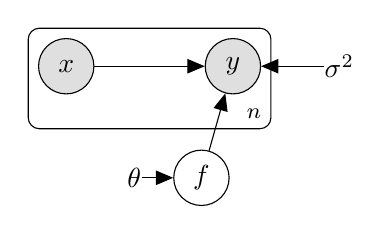
\begin{tikzpicture}
    \node[obs] (y) {$y$};
    \node[latent, below=0.7 of y, xshift=-0.4cm] (f) {$f$};
    \node[obs, left=of y, xshift=-0.4cm]  (x) {$x$};
    \node[const, right=of y, xshift=-0.2cm]  (sigma) {$\sigma^2$};
    \node[const, left=0.4 of f] (theta) {$\theta$};

    % Connect the nodes
    \edge {x, f, sigma} {y} ; %
    \edge {theta} {f} ; %

    % Plates
    \plate {yx} {(x)(y)} {$n$} ;
  \end{tikzpicture}

  \caption{Gaussian Process plate diagram.\label{fig:gp_plate} }
\end{figure}


In this model, the posterior of $f$ is available analytically, by virtue of
Gaussian-Gaussian conjugacy. Consider evaluating the function $f$ at new points
$x_{\ast}$, denoted by $f_{\ast} := f\left(x_{\ast}\right)$. Then, the joint of
$y$ and $f^{\ast}$ is
\begin{align*}
  \begin{pmatrix}
    y \\ f_{\ast}
  \end{pmatrix} &= \Gsn\left(
 \begin{pmatrix}
   0 \\ 0
 \end{pmatrix} ,
\begin{pmatrix}
  K\left(x, x\right) + \sigma^{2}I_{n} & K\left(x, x_{\ast}\right) \\
  K\left(x_{\ast}, x\right) & K\left(x_{\ast}, x_{\ast}\right)
\end{pmatrix}
  \right),
\end{align*}
which yields the posterior,
\begin{align*}
  f_{\ast} \vert y &\sim \Gsn\left(\Earg{f_{\ast} \vert y}, \Covarg{f_{\ast} \vert y}\right),
\end{align*}
where
\begin{align*}
  \Earg{f_{\ast} \vert y} &= K\left(x_{\ast}, x\right)\left(K\left(x, x\right) + \sigma^{2}I_{n}\right)^{-1}y \\
  \Covarg{f_{\ast} \vert y} &= K\left(x_{\ast}, x_{\ast}\right) - K\left(x_{\ast}, x\right)\left(K\left(x, x\right) + \sigma^{2}I_{n}\right)^{-1}K\left(x, x_{\ast}\right)
\end{align*}

Note the $n\times n$ matrix inversion in the covariance calculation. This is the
source of the $O\left(n^{3}\right)$ complexity of using standard GPs, though a
variety of fast approximations have been proposed, exploiting the sparse,
banded, or block structure within the covariance
\citep{quinonero2007approximation}.

In this computation, we have assumed the the kernel hyperparameters $\theta$ is
known\footnote{For example, in the Gaussian covariance case, this has the form
  $\theta = \left(\sigma_{f}^{2}, M\right)$}. In reality, these must be inferred
from the data. Two standard approaches are based on maximizing (1) the marginal
likelihood of $y$ and (2) the cross-validated predictive likelihood. The first
approach leverages the fact that the marginal likelihood,
\begin{align*}
\log p\left(y \vert x; \theta\right) &= -\frac{n}{2}\log 2\pi - \log\absarg{K_{\theta}\left(x, x\right) + \sigma^{2}I_{n}} - \frac{1}{2}y^{T}\left(K_{\theta}\left(x, x\right) + \sigma^{2}I_{n}\right)^{-1}y
\end{align*}
and its gradients over $\theta$ have a closed form, and so can be optimized.

The cross-validation approach instead maximizes the average predicted log probability,
\begin{align*}
\sum_{i = 1}^{n} \log p\left(y_{i} \vert x, y_{-i}; \theta\right),
\end{align*}
which can also be found analytically, by conditioning the marginal for $y$.

- Review GP graphical model
- Basic distinctions from previous models
- Description of GP posterior
  + GP pseudocode
  + Link to some actual code

\subsection{Linear dynamical systems}
\label{subsec:linear_dynamical_systems}

Linear dynamical systems model an observed time series as a transformation of
temporally evolving latent states. The basic idea reminds me of trying to swat a
fly. I might hear a buzzing noise, which gives some sense of where the fly is,
and I might know that it can't move too far too quickly, but I might only get a
few brief glimpses of the actual insect. The evolving latent state here is the
true position of the fly, while the transformation that we observe is the
loudness of the buzzing. There have been many proposals that allow general
transformation and state evolution behavior, but a fundamental starting point is
the linear-gaussian dynamical system,

\begin{align*}
  z_{t} &= A z_{t - 1} + \eps_{t} \\
  x_{t} &= C z_{t} + \delta_{t} \\
  w_{t} &\sim \Gsn\left(0, Q\right) \\
  \eps_{t} &\sim \Gsn\left(0, R\right).
\end{align*}

The $z_{t}$'s are a markov chain of latent states, while the $x_{t}$'s represent
the observed emissions from it. $A$ and $\Lambda$ govern the dynamics of the
underlying process, while $C$ and $\Sigma$ describe the emission structure. The
associated graphical model is provided in Figure \ref{fig:lds_graphical}.

There are two conceptual components to fitting this model,

\begin{itemize}
\item Inference: Even if $\Theta = \{A, C, Q, R\}$ were known, there
  is often value in estimating the latent $z_{i}$.
\item Learning: Typically, the parameters $\Theta$ are unknown, and must
  themselves be learned from the data.
\end{itemize}

Further, inference can be approached in several different ways, depending on
problem context and constraints. Among the most common approaches are

\begin{itemize}
\item Filtering: Update beliefs of the current latent state in an online
  fashion. Quantitatively, the goal is to estimate the distribution
  $p\left(z_{t} \vert x_{1:t}\right)$.
\item Smoothing: Use the full history to estimate beliefs of each latent state,
  one at a time. This means to estimate $p\left(z_{t} \vert x_{1:T}\right)$ for
  each $t = 1, \dots, T$.
\item Forecasting: Predict the next few latent states given all observations so
  far. For example, we might be interested in $p\left(z_{t + 1} \vert
  x_{1:t}\right)$.
\end{itemize}

\begin{figure}[ht]
  \centering
  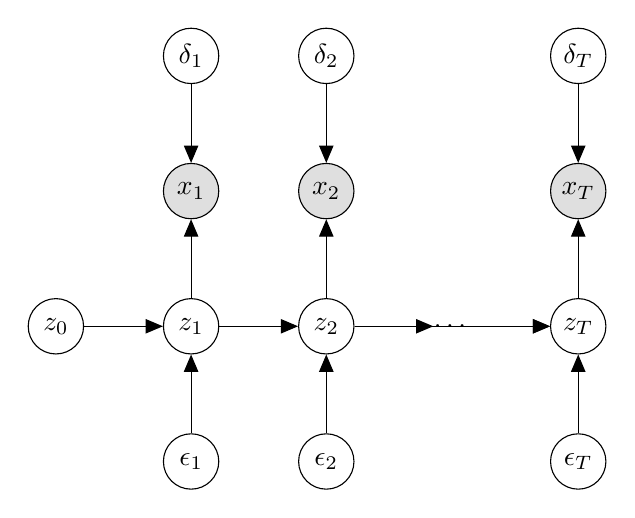
\begin{tikzpicture}
    \node[latent] (z1) {$z_{1}$};
    \node[latent, left=of z1] (z0) {$z_{0}$};
    \node[obs, above=of z1] (x1) {$x_{1}$};
    \node[latent, above=of x1] (delta1) {$\delta_{1}$};
    \node[latent, below=of z1] (eps1) {$\eps_{1}$};
    \node[latent, right=of z1] (z2) {$z_{2}$};
    \node[obs, above=of z2] (x2) {$x_{2}$};
    \node[latent, above=of x2] (delta2) {$\delta_{2}$};
    \node[latent, below=of z2] (eps2) {$\eps_{2}$};
    \node[const, right=of z2] (zdots) {$\dots$};
    \node[latent, right=of zdots] (zT) {$z_{T}$};
    \node[latent, below=of zT] (epsT) {$\eps_{T}$};
    \node[obs, above=of zT] (xT) {$x_{T}$};
    \node[latent, above=of xT] (deltaT) {$\delta_{T}$};

    % Connect the nodes
    \edge {z1} {x1} ; %
    \edge {z2} {x2} ; %
    \edge {z0} {z1} ; %
    \edge {z1} {z2} ; %
    \edge {z2} {zT} ; %
    \edge {z2} {zdots} ; %
    \edge {zdots} {zT} ; %
    \edge {zT} {xT} ; %
    \edge {eps1} {z1} ; %
    \edge {eps2} {z2} ; %
    \edge {epsT} {zT} ; %
    \edge {delta1} {x1} ; %
    \edge {delta2} {x2} ; %
    \edge {deltaT} {xT} ; %
  \end{tikzpicture}
  \caption{\label{fig:lds_graphical} }
\end{figure}

We first describe inference in detail, before describe how inference and
learning can be alternated to fit models on real data. Due to the linear
gaussian assumption, the conditionals required by filtering and smoothing are
still gaussian; however, their means and covariances are not immediately
apparent. It turns out that, for both filtering and smoothing, they can be
efficiently computed via dynamic programming recursions. In the literature,
these are referred to as the Kalman Filtering and Rauch-Tung-Striebel Smoothing
recursions.

Consider the filter, where the goal is inference of $p\left(z_{t} \vert
x_{1:t}\right)$. We will assume $z_{1} \sim \Gsn\left(0, Q\right)$. We
could alternatively fix it to a constant -- the point is that the distribution
for $z_{1}$ is known.

For $t > 1$, define the \textit{one-step-ahead} and \textit{updated} means and
covariances by
\begin{align*}
  \mu_{t \vert t - 1} &:= \Earg{z_{t} \vert y_{1:t - 1}} \\
  \Sigma_{t \ vert t - 1} &:= \Covarg{z_{t} \vert y_{1:t - 1}} \\
  \mu_{t} &:= \Earg{z_{t} \vert y_{1:t}} \\
  \Sigma_{t} &:= \Covarg{z_{t} \vert y_{1:t}}.
\end{align*}

The update means and covariances $\mu_{t}$ and $\Sigma_{t}$ are the main
quantities of interest in filtering. The filtering algorithm is detailed in in
Algorithm \ref{alg:kalman_filter}. It can be thought of as a forwards pass
through the observed sequence, updating means and covariances along the way.

The derivation is as follows. For the predict step, use teh tower property and
the law of total variance,

\begin{align*}
  \Earg{z_{t} \vert y_{1:t - 1}} &= \Earg{\Earg{z_{t} \vert z_{t - 1}, y_{1:t - 1}}} \\
  & = \Earg{Az_{t - 1}\vert y_{1:t - 1}} \\
  &= A\mu_{t - 1} \\
  \Covarg{z_{t} \vert y_{1:t - 1}} &= \Covarg{\Earg{z_{t} \vert z_{t - 1}, y_{1:t - 1}}} + \Earg{\Covarg{z_{t} \vert z_{t - 1}, y_{1:t - 1}}} \\
  &= \Covarg{Az_{t - 1} \vert z_{t - 1}, y_{1:t - 1}} + \Earg{Q} \\
  &= A\Sigma_{t - 1}A^{T} + Q.
\end{align*}

For the update step, use gaussian conjugacy to obtain the required means and
covariances and the matrix inversion lemma to express them more concisely.
More precisely,

\begin{align*}
p\left(z_{t} \vert x_{1:t}\right) \propto p\left(x_{t} \vert z_{t}\right)p\left(z_{t} \vert y_{1:t}\right),
\end{align*}
and both densities on the right are gaussian -- the first is the likelihood of
the observed $x_{t}$ while the second is the predict density derived above. By
Bayes' rule, the posterior is gaussian with increased precision,
\begin{align}
  \label{eq:sigma_t_inv}
\Sigma_{t}^{-1} &= \Sigma_{t \vert t - 1}^{-1} + C^{T}R^{-1}C
\end{align}
and shrunken mean,
\begin{align}
  \label{eq:mu_t}
\mu_{t} &= \Sigma_{t}CR^{-1}x_{t} + \Sigma_{t}\Sigma_{t \vert t - 1}^{-1} \mu_{t \vert t - 1}.
\end{align}

Recall the matrix inversion lemma,
\begin{align*}
\left(A + UCV\right)^{-1} &= A^{-1} + A^{-1}U\left(C^{-1} + VA^{-1}U\right)^{-1}VA^{-1},
\end{align*}
and apply it to equation \ref{eq:sigma_t_inv} to find
\begin{align*}
  \Sigma_{t} &= \Sigma_{t \vert t - 1} - \Sigma_{t \vert t - 1}C\left(R^{-1} + C \Sigma_{t \vert t - 1}C^{T}\right)^{-1}C\Sigma_{t \vert t - 1} \\
  &= \left(I - K_{t}C\right)\Sigma_{t \vert t - 1},
\end{align*}
according to the definition of $K_{t}$ in Algorithm
\ref{algorithm:kalman_filter}.

Substituting this expression, we can simplify equation \ref{eq:mu_t},
\begin{align*}
  \mu_{t} &= \left(I - K_{t} C\right)\Sigma_{t \vert t - 1}\left(C R^{-1}x_{t} + \Sigma_{t \vert t - 1}^{-1} \mu_{t \vert t - 1}\right) \\
  &= \left(I - K_{t}C\right)\mu_{t \vert t - 1} + \left(I - K_{t} C\right)\Sigma_{t \vert t - 1}C R^{-1} x_{t} \\
  &= \mu_{t \vert t - 1} + K_{t}\left(x_{t} - C\mu_{t \vert t- 1}\right),
\end{align*}
where for the simplification on the second half of the second line,
\begin{align*}
  \left(I - K_{t}C\right)\Sigma_{t \vert t - 1} C R^{-1} x_{t} &= \left(I - \left(\Sigma_{t \vert t - 1}^{-1} + C^{T} R C\right)^{-1}C^{T}R^{-1}C\right)\Sigma_{t \vert t - 1}C R^{-1} x_{t} \\
  &= K_{t}x_{t},
\end{align*}
we again used the matrix inversion lemma.

\begin{algorithm}
   \caption{The Kalman filtering predict-update recursions.}
   \label{alg:kalman_filter}
\begin{algorithmic}
  \STATE {\bfseries Input:} Model parameters $\Theta = \{A, C, Q, R\}$ and
    observed sequence $x_{1:T}$.
    \STATE $\mu_{0} \leftarrow 0, \Sigma_{0} \leftarrow Q$ \hfill initialize distribution of
    $z_{0}$.
    \FOR{$t = 1 \dots T$}
    \STATE $\mu_{t \vert t - 1} \leftarrow A\mu_{t - 1}$ \hfill predict step
    \STATE $\Sigma_{t \vert t - 1} \leftarrow A \Sigma_{t - 1} A^{T} + Q$
    \STATE $\mu_{t} \leftarrow \mu_{t \vert t - 1} + K_{t}\left(x_{t} - C\mu_{t \vert t - 1}\right)$ \hfill update step
    \STATE $\Sigma_{t} \leftarrow \left(I - K_{t}C\right)\Sigma_{t \vert t - 1}$
    \STATE where $K_{t} \leftarrow \left(\Sigma_{t \vert t - 1}^{-1} + C^{T}R C\right)^{-1} C^{T}R^{-1}$
    \ENDFOR
    \STATE {\bfseries Output:} Filtered means and covariances $\left(\mu_{t},
    \Sigma_{t}\right)_{t = 1}^{T}$.
\end{algorithmic}
\end{algorithm}

While the Kalman filter makes a forwards pass over the observations to estimate
the latent state means and covariances as data are made available, the RTS
smoother can be understood as a pair of forwards-backwards sweeps that
propogates information from all observations to the latent state estimates at
previously measured timepoints. Introduce the notation,

\begin{align*}
\mu_{t \vert T} &= \Earg{z_{t} \vert y_{1:T}} \\
\Sigma_{t \vert T} &= \Covarg{z_{t} \vert y_{1:T}},
\end{align*}

Which completely determine the smoothed distributions $p\left(z_{t} \vert
x_{1:T}\right)$ of interest. The forwards pass in RTS smoothing is identical to
the Kalman filter, and pseudocode for the backwards pass is provided in
Algorithm \ref{alg_kalman_smoother}.

\begin{algorithm}
   \caption{The Kalman smoothing backwards pass.}
   \label{alg:kalman_smoother}
\begin{algorithmic}
  \STATE {\bfseries Input:} Model parameters $\Theta = \{A, C, Q, R\}$,
    observed sequence $x_{1:T}$, and filtering quantities $\left(\mu_{t},
    \Sigma_{t}, \mu_{t \vert t - 1}, \Sigma_{t \vert t - 1}\right)$
    \STATE $\mu_{T \vert T} \leftarrow \mu_{T}, \Sigma_{T \vert T} \leftarrow
    \Sigma_{T}$ \hfill initialize distribution of $z_{T}$ using the results from
    the Kalman filter.
    \FOR{$t = T - 1 \dots 1$}
    \STATE $\mu_{t \vert T} \leftarrow \mu_{t} + J_{t}\left(\mu_{t + 1 \vert T} - \mu_{t + 1 \vert t}\right)$
    \STATE $\Sigma_{t \vert T} \leftarrow \Sigma_{t} + J_{t}\left(\Sigma_{t + 1 \vert T} - \Sigma_{t + 1 \vert t}\right)J_{t}^{T}$
    \STATE where $J_{t} \leftarrow \Sigma_{t \vert t}A_{t + 1}^{T} \Sigma_{t + 1\vert t}^{-1}$
    \ENDFOR
    \STATE {\bfseries Output:} Smoothed means and covariances $\left(\mu_{t \vert T},
    \Sigma_{t \vert T}\right)_{t = 1}^{T}$.
\end{algorithmic}
\end{algorithm}

To see why this update works, first consider the joint behavior of neighboring
times,

\begin{align*}
   \left(z_{t}, z_{t + 1} \vert x_{1:t}\right) &\sim \Gsn\left(
\begin{pmatrix}
  \mu_{t \vert t} \\
  \mu_{t + 1 \vert t}
\end{pmatrix},
\begin{pmatrix}
  \Sigma_{t \vert t} & \Sigma_{t} A^{T} \\
  A \Sigma_{t} & \Sigma_{t + 1 \vert t}
\end{pmatrix}\right),
\end{align*}
because
\begin{align*}
\Covarg{z_{t}, z_{t + 1} \vert x_{1:t}} &= \Covarg{z_{t}, Az_{t} + \eps_{t + 1} \vert x_{1:t}} \\
&= \Sigma_{t}A^{T}.
\end{align*}

Conditioning, we obtain
\begin{align*}
  z_{t} \vert z_{t + 1}, x_{1:t} &\sim \Gsn\left(
  z_{t} \vert \mu_{t \vert t} + J_{t}\left(z_{t + 1} - \mu_{t + 1 \vert t}\right),
  \Sigma_{t \vert t} - J_{t} \Sigma_{t + 1 \vert t} J_{t}^{T}
  \right).
\end{align*}
Since $x_{t}$ is independent of $x_{(t + 1): T}$ conditional on $z_{t + 1}$,
this is enough to compute the full smoothed means and covariances. By the tower
property,
\begin{align*}
  \mu_{t \vert T} &= \Earg{z_{t} \vert x_{1:T}} \\
  &= \Earg{\Earg{z_{t} \vert z_{t + 1}, x_{1 : T}} \vert x_{1:T}} \\
  &= \Earg{\Earg{z_{t} \vert z_{t + 1}, x_{1:t}} \vert x_{1:T}} \\
  &= \mu_{t \vert t} + J_{t}\left(\mu_{t + 1 \vert T} - \mu_{t + 1 \vert t}\right)
\end{align*}
and similarly by the law of total covariance,
\begin{align*}
  \Sigma_{t\vert T} &= \Covarg{z_{t} \vert x_{1:T}} \\
  &= \Covarg{\Earg{z_{t} \vert z_{t + 1}, x_{1:T}}} + \Earg{\Covarg{z_{t} \vert z_{t + 1}, x_{1:T}}} \\
  &= \Covarg{\Earg{z_{t} \vert z_{t + 1}, x_{1:t}}} + \Earg{\Covarg{z_{t} \vert z_{t + 1}, x_{1:t}}} \\
  &= \Sigma_{t \vert t} + J_{t}\left(\Sigma_{t + 1 \vert T} - \Sigma_{t + 1 \vert t}\right) J_{t}^{T}
\end{align*}

\section{Temporal mixture models}
\label{sec:temporal_mixture_models}

In all the models considered so far, all time windows exhibit comparable
behavior. In the problem description of section \ref{sec:problem_description}
however, we would expect changes in the behavior of the system during different
temporal regimes. In this section, we describe probabilistic models that
generate this sort of behavior. The unifying probabilistic ``trick'' that helps
accomplish this goal is the introduction of latent variables specying which
regime the system is in at any given timepoint.

\subsection{Hidden Markov Modeling}

The idea behind Hidden Markov Models (HMMs) is similar to that of LDSs, with the
exception that the $z_{t}$ are no longer thought of as continuous latent
variables. Instead, each $z_{t}$ is assigned one of a few discrete states,
which switch between one another according to a Markov chain.

An informal analogy is how I choose to listen to different music tracks. For a
few days, I might be mostly listening to sonatas by Beethoven and Schubert,
because I'm in a latent state that prefers German piano sonatas. I might be more
likely to transition from here to French chamber music than, say, LA punk. So,
my underlying style preferences evolve according to a Markov chain $z_{t}$,
which is in turn reflected by the actual tracks $x_{t}$ that I listen to.

More formally, we suppose $z_{1} \sim \pi_{0}$ comes from some initial
distribution $\pi_{1} \in \simplex^{K - 1}$ and has some $K \times K$ transition
probability matrix $P$ whose rows lie in $\simplex^{K - 1}$, where $\simplex^{K
  - 1}$ denotes the $K - 1$ dimensional simplex. Conditional on $z_{t}$, $x_{t}$
is emitted according to the density $p_{\theta_{z_{t}}}\left(x\right)$, one of
$K$ emission densities $p_{\theta_{1}}\left(x\right), \dots,
p_{\theta_{k}}\left(x\right)$. Concisely,
\begin{align*}
  x_{t} \vert z_{t} &\sim p_{\theta_{z_{t}}} \\
  z_{1} &\sim \pi_{1} \\
  z_{t} \vert z_{t - 1} &\sim P_{z_{t - 1}, z_{t}} \text{ for } t > 1.
\end{align*}

As in LDSs, fitting this model can be broken into an inference and a learning
step, which estimate the distributions of the $z_{t}$ conditional on observed
data and which fit the model parameters $\{P, \pi, \theta_{1}, \dots,
\theta_{K}\}$. Alternating these two steps optimizes the Expected Complete Data
Loglikelihood in an EM algorithm.

The latent state inference (the $E$-step) is referred to as the
Forwards-Backwards algorithm. This procedure parallels the Kalman filter
(Forwards) and smoother (Backwards) algorithm for inference in LDSs. First,
we find a simple expression for the analog of the filtered densities, based on
the Markov assumption on the $z_{t}$'s,
\begin{align*}
  p\left(z_{t} \vert x_{1:t}\right) &\propto p\left(x_{t} \vert z_{t}, x_{1:t - 1}\right) p\left(z_{t} \vert x_{1:t - 1}\right) \\
  &= p\left(x_{t} \vert z_{t}\right) p\left(z_{t} \vert x_{1:t - 1}\right) \\
  &= p_{\theta_{z_{t}}}\left(x_{t}\right)p\left(z_{t} \vert x_{1:t - 1}\right).
\end{align*}
The first term is known by assumption, while the second can be computed directly
from the previous filtered probabilities,
\begin{align*}
  p\left(z_{t} \vert x_{1:t - 1}\right) &= \sum_{k = 1}^{K} p\left(z_{t} \vert z_{t - 1} = k\right)p\left(z_{t - 1} = k \vert x_{1:t - 1} \right).
\end{align*}

The forwards pass of the Forwards-Backwards algorithm alternates these two steps
(``update'' and ``predict''), after initializing $p\left(z_{1}\right) =
\pi_{1}$, as described in algorithm \ref{alg:hmm_forwards}.

\begin{algorithm}
   \caption{Safe log-sum-exp}
   \label{alg:normalize_log}
   \begin{algorithmic}
     \STATE {\bfseries Input:} $x \in \reals^{n}$
     \STATE $m \leftarrow \max\left(x\right)$
     \STATE {\bfseries Output:} $lse\left(x\right) \leftarrow x - \left(m + \log\left(\sum\exp{x_{i} - m}\right)\right)$
   \end{algorithmic}
\end{algorithm}

\begin{algorithm}
   \caption{Forwards pass for HMM Inference}
   \label{alg:hmm_forwards}
\begin{algorithmic}
  \STATE {\bfseries Input:} Model parameters $\{\pi_{1}, P, \theta_1, \dots, \theta_K\}$,
  observed sequence $x_{1:T}$
  \STATE $\log \tilde{p}\left(z_{1}\vert x_{1}\right) \leftarrow
  \log\pi_{1} + \begin{pmatrix} \log p_{\theta_{1}}\left(x_{1}\right) \\ \vdots \\ \log p_{\theta_{k}}\left(x_{1}\right) \end{pmatrix}$ \hfill initialize distribution of $z_{1}$
  \STATE $\log p\left(z_{1} \vert x_{1}\right) \leftarrow \log \tilde{p}\left(z_{t} \vert x_{1}\right) - \text{lse}\left(\log \tilde{p}\left(z_{t} \vert x_{1}\right)\right)$\hfill Use algorithm \ref{alg:normalize_log}
  \FOR{$t = 2 \dots T$}
  \STATE $\log \tilde{p}\left(z_{t} \vert x_{1:t}\right) \leftarrow P \exp{\log p\left(z_{t - 1} \vert x_{1:t - 1}\right)} + \begin{pmatrix}  \log p_{\theta_{1}}\left(x_{t}\right) \\ \vdots \\ \log p_{\theta_{k}}\left(x_{t}\right) \end{pmatrix}$
  \STATE $\log p\left(z_{1} \vert x_{1:t}\right) \leftarrow \log \tilde{p}\left(z_{t} \vert x_{1:t}\right) - \text{lse}\left(\log \tilde{p}\left(z_{t} \vert x_{1:t}\right)\right)$\hfill
  \ENDFOR
  \STATE {\bfseries Output:} Filtered log densities $\log p\left(z_{t} \vert x_{1:t}\right)$.
\end{algorithmic}
\end{algorithm}

\begin{algorithm}
  \begin{algorithmic}
   \caption{Backwards pass for HMM Inference}
   \label{alg:hmm_backwards}
   \STATE {\bfseries Input:} Model parameters $\{\pi_{1}, P, \theta_1, \dots, \theta_k\}$, observed sequence $x_{1:T}$
   \STATE $\log p\left(z_{T} \vert x_{1:T}\right) \leftarrow 0_{K}$ \hfill Initialize messages.
   \FOR{$t = T  - 1\dots 1$}
   \FOR{$k = 1 \dots K$}
   \STATE $\log p\left(z_{t} = k \vert x_{1:T}\right) \leftarrow \text{lse}\left(\log p\left(z_{t + 1} = k \vert x_{1:T}\right)\right) + \log p_{\theta_{k}}\left(y_{t}\right) + \log \pi_{k}$
   \ENDFOR
   \ENDFOR
   \STATE {\bfseries Output:} Smoothed densities $\log p\left(z_{t} \vert x_{1:T}\right)$.
  \end{algorithmic}
\end{algorithm}

The backwards pass computes the analog of the smoothed densities, based on the
observation\footnote{This is the same observation used in the derivation of the
  Kalman smoother.} that $x_{t}$ is independent of the future conditional on
$z_{t + 1}$,
\begin{align*}
  p\left(z_{t} \vert x_{1:T}\right) &\propto p\left(x_{t + 1:T} \vert z_{t}\right) p\left(z_{t} \vert x_{1:t}\right).
\end{align*}
The second term on the right hand side is available from the forwards pass. The
first term is computed during the backwards pass, which initializes $p\left(x_{T
  + 1} \vert z_{T}\right) = 1$ and then accumulates the ``future observation''
densities from right to left,
\begin{align*}
  p\left(x_{t + 1: T} \vert z_{t}\right) &= \sum_{k = 1}^{K} p\left(z_{t + 1} = k, x_{t + 1 : T} \vert z_{t}\right) \\
  &= \sum_{k = 1}^{K} p\left(x_{t + 2: T}\vert z_{t + 1} = k, x_{t + 1}, z_{t}\right) p\left(z_{t + 1} = k, x_{t + 1} \vert z_{t}\right) \\
  &= \sum_{k = 1}^{K} p\left(x_{t + 2:T}\vert z_{t + 1} = k\right)p_{\theta_{z_{t + 1}}}\left(x_{t + 1}\right) \P_{z_{t}, k}.
\end{align*}

The backwards pass is summarized in algorithm \ref{alg:hmm_backwards}.

In the learning step, the parameters $\left(\theta_{k}\right)$, $\pi_0$ and
$\pi_{k, k^{\prime}}$ must be estimated. Estimation of the per-regime parameters
can be done separately for each $k$. For example, if HMM has Gaussian emissions,
$p_{\theta_{k}}\left(x_{t}\right) = \Gsn\left(x_{t} \vert \mu_{k},
\Sigma_{k}\right)$, then
\begin{align*}
  \hat{\mu}_{k} &= \frac{\sum_{t = 1}^{T} \indic{z_{t} = k}x_{t}}{\sum_{t = 1}^{T}\indic{z_{t} = k}} \\
  \hat{\Sigma}_{k} &= \frac{\sum_{t = 1}^{T} \indic{z_{t} = k}\left(x_{t} - \hat{\mu}_{k}\right)\left(x_{t} - \hat{\mu}_{k}\right)^{T}}
      {\sum_{t = 1}^{T} \indic{z_{t} = k}},
\end{align*}
while, regardless of the emission structure, the Markov chain parameters can be
estimated via
\begin{align*}
  \hat{\pi}_{k, k^{\prime}} &= \frac{\sum_{t = 1}^{T} \indic{z_{t} = k, z_{t + 1} = k^{\prime}}}{\sum_{t = 1}^{T} \indic{z_{t} = k}}.
\end{align*}

- Probabilistic approach that incorporates time structure directly
- Draw the graphical model
- Write the model and provide an interpretation

\subsubsection{HMM for for antibiotics}
\label{subsubsec:hmm_for_antibiotics}

In the context of regime detection in the microbiome, we imagine a few
underlying states shared across all bacteria (ranging from high abundance to
complete absence). Within each species, states evolve independently according to
a Markov chain. Note that, while we do share across species when estimating
underlying parameters $\left(\theta_{k}\right)$, we do not tie together latent
indicators $z_{it}$ across species. Specifically, we use a DAG that factors
across all species -- given $\theta$, all species abundances follow independent
HMMs.

Therefore, in the $E$-step (Forwards-Backwards algorithm), the $z_{it}$ can be
estimated in parallel across all species. The $M$-step is modified so that
mixture component parameters and transition probabilities are estimated
simultaneously across all species, for example, the new mean update for cluster
$k$ in the Gaussian HMM becomes
\begin{align*}
\hat{\mu}_{k} &= \frac{\sum_{i = 1}^{n}\sum_{t = 1}^{T} \indic{z_{t} = k}x_{it}}{\sum_{i = 1}^{n}\sum_{t = 1}^{T} \indic{z_{it} = k}}.
\end{align*}

Next, we employ this approach on the same antibiotics data described in section
\ref{subsubsec:antibiotics_application}. The results are summarized in Figure
\ref{fig:hmm_mode} and Supplementary Figure \ref{fig:hmm_probs}, which display
the modes and raw probabilities of the smoothed probabilities $p\left(z_{it}
\vert x_{i(1:T)}\right)$ after applying EM. As in Figure
\ref{fig:centroid-euclidean-conditional} and its counterparts made through
hierarchical clustering, rows correspond to individual species, while columns
are samples sorted by time. The three main panels are the three subjects in the
study. Here, rows $i$ are ordered according to a hierarchical clustering on the
estimated model sequences $\left(\hat{z}_{i1}, \dots, \hat{z}_{iT}\right)$,
where $\hat{z}_{it} = \arg \max_{k} p\left(z_{it} = k \vert x_{1:T}\right)$. The
intensity of the shading of each cell corresponds to the average value
$\hat{\mu}_{k}$ for that mode.

We can think of Figure \ref{fig:hmm_mode} as a smoothed version of the raw
heatmaps made through hierarchical clustering. By coarsening the raw values into
cluster centers, certain patterns are more easily visible. For example, in
addition to effect of the two antibiotics time courses across all subjects, we
note that

\begin{itemize}
\item The effect of the first antibiotic time courses is more prolonged in
  Subject F, and in some cases species disappear for most of the remainder of
  the experiment. Some of these species seem to have also disappeared from
  Subject D, but most others recovered in both Subject D and E.
\item The phenomenon in which some species become \textit{more} abundant during
  the time courses -- presumably filling in newly emptied niches -- is stronger
  in Subject E than the others. Further, some species that exhibit this behavior
  in Subject E respond differently within subjects D and F, becoming less
  abundant rather than more.
\end{itemize}

Note that, while smoothing makes the antibiotic effect clearer among moderately
and highly abundant species, variation among rarer species, to which all
timepoints are assigned to the rare abundance state, is obscured. This could be
remedied by increasing $K$, at the cost of increasing the complexity of
interpretation for abundant species.

Instead of displaying the sequence of modes $\hat{z}_{it}$, Supplemental Figure
\ref{fig:hmm_probs} provides the individual probabilities $p\left(z_{it} = k
\vert x_{1:T}\right)$ across $k$. The vertical panels distinguish between
different $k$, while transparency represents the size of the probability --
smaller probabilities are more transparent. The colors are associated with
centroid means, as before. In this application, most probabilities seem near
one, so this view adds little to that in \ref{fig:hmm_mode}. However, this does
suggest the possibility of overfitting, which we address by introducing priors
on $\Theta$ in section \ref{sec:sticky_hmms}.

The estimated transition probabilities between states, ordered in terms of
increasing $\hat{\mu}_{k}$, are displayed below.
\begin{verbatim}
      1     2     3     4
1 0.810 0.159 0.028 0.003
2 0.389 0.527 0.083 0.002
3 0.077 0.094 0.810 0.019
4 0.027 0.007 0.056 0.910
\end{verbatim}
Unsurprisingly, most transitions remain in the same state, and any departures
are generally restricted to states with similar $\hat{\mu}_{k}$s. Generally,
there appear to be more transitions downwards than upwards, and the sum of
transitions into state 1 is higher than the sums for the rest. This can likely
be attributed to the antibiotic effect, which reduces abundances of species that
often never recover.

As in Figure \ref{fig:centroid-euclidean-conditional}, the primary drawback of
this display is the difficulty in linking observed species trajectories to
species or taxonomic detail. To easily link the smoothed HMM estimates to raw
time series values and species descriptions would require either splitting the
view across taxonomies or introducing interactivity.

- Application to antibiotics: heatmap, interpretation, and transition
probability matrix
- In order to understand extensions, briefly review actual inferential mechanism
- What kinds of limitations have we encountered?

\begin{figure}[ht]
  \centering
  \includegraphics[width=0.9\textwidth]{figure/hmm_mode}
  \caption{The modal sequences according to the HMM estimated through
    EM. \label{fig:hmm_mode} }
\end{figure}

\subsubsection{Sticky HMMs}
\label{sec:sticky_hmms}

Sticky HMMs are an extension of ordinary HMMs designed to incorporate
additional ``stickiness'' into state transitions -- states should be encouraged
remain unchanged over longer sequences. To practically implement this basic
idea, a bayesian view is useful, and we describe inference in detail. An
application to the antibiotics data concludes this section.

Consider the standard Bayesian HMM, which places $\Dir\left(\alpha\right)$
priors on the rows of the transition probability matrix, $P_{1}, \dots, P_{K}$
and conjugate priors on $\Theta$. The main idea of the sticky HMM is to
introduce a ``stickiness'' parameter $\kappa$ to the Dirichlet
prior\footnote{Here, $e_{k} := \left(0, \dots, 0, 1, 0, \dots, 0\right)$ is the
  vector with a $1$ in the $k^{th}$ coordinate and zeros everywhere else.}:
$P_{k} \sim \Dir\left(P_{k} \vert \alpha + \kappa e_{k}\right)$. This means that
draws from the prior on $P$ will have larger weight along the diagonal,
depending on the size of $\kappa$, and since diagonal elements correspond to
self-transitions, chains drawn from the prior will be ``sticky.''

To draw samples from $p\left(\left(z_{it}\right), P, \Theta \vert
\left(x_{it}\right)\right)$, we consider a block gibbs sampling analog to EM
\citep{fruhwirth2006finite}. In place of the $E$-step, we draw from the
conditional $p\left(\left(z_{it}\right) \vert \left(x_{it}\right),
\Theta\right)$ using a variation of the forwards-backwards algorithm, and in
place of the $M$-step, we draw from $p\left(\Theta, \vert P, \left(z_{it}\right),
\left(x_{it}\right)\right)$ and $p\left(P \vert \Theta, \left(z_{it}\right),
\left(x_{it}\right)\right)$. We generally follow the derivation of
\citep{fox2009bayesian}.

First we consider sampling $p\left(\left(z_{it}\right) \vert P, \Theta\right)$.
Note that since each sequence is independent of all others, given $\Theta$, we
can sample the $z_{it}$ separately across each $i$, so for the explanation
below, we drop this subscript. By the Markov property, the probability a single
sequence can be decomposed according to
\begin{align}
  \label{eq:sticky_block_z}
p\left(z_{1:T} \vert x_{1:T}, \Theta, \pi, P\right) &= p\left(z_{1} \vert y_{1:T}, \Theta, \pi, P\right) \prod_{t = 2}^{T} p\left(z_{t} \vert z_{t - 1}, y_{1:T}, \Theta, \pi, P\right).
\end{align}
If we could calculate each of these individual probabilities, then one mechanism
for sampling the entire sequence $z_{1:T}$ would be to first sample $z_{1}$,
then $z_{2}$ given $z_{1}$, etc. Note that the first term has a different
structure than the rest (it doesn't depend on any previous $z_{t}$s), so we
analyze it first,
\begin{align*}
  p\left(z_{1} \vert y_{1:T}, \Theta, \pi, P\right) &\propto p\left(z_{1} \vert \Theta, \pi, P\right) p\left(y_{1} \vert z_{1}, \Theta, \pi, P\right) p\left(y_{2:T} \vert z_{1}, \Theta, \pi, P\right) \\
  &\propto \pi_{z_{1}} p\left(y_{1} \vert \theta_{z_{1}}\right) p\left(y_{2:T} \vert z_{1}, \Theta, \pi, P\right)
\end{align*}
where we used the fact that $y_{1} \independent y_{2:T} \vert z_{1}$, due to the
structure of the HMM DAG. The first two terms are easy to sample, and we will
show below that terms of the form $p\left(y_{t + 1:T} \vert z_{t}, \Theta, \pi,
P\right)$ can be calculated efficiently using a backwards-pass type recursion.

Consider now the terms in the product of equation \ref{eq:sticky_block_z}. By
Bayes rule,
\begin{align*}
  p\left(z_{t} \vert z_{t - 1}, y_{1:T}, \Theta, \pi, P\right) &\propto p\left(y_{1:t - 1} \vert z_{t - 1}, z_{t}, \Theta, \pi, P\right)
  p\left(y_{t} \vert z_{t}, \Theta, \pi, P\right)
  p\left(y_{t + 1 : T} \vert z_{t}, \Theta, \pi, P\right) \\
  &\propto p\left(y_{1:t - 1} \vert z_{t - 1}, z_t, \Theta, \pi, P\right) p\left(y_t \vert \theta_{z_t}\right) p\left(y_{t + 1 : T}\vert z_{t}, \Theta, \pi, P\right).
\end{align*}
The second term is a likelihood, and the third will be calculated by the
backwards-pass. Note that the first term can be further reduced to
\begin{align*}
  p\left(y_{1:t - 1} \vert z_{t - 1}, z_t, \Theta, \pi, P\right) &\propto p\left(z_{t} \vert y_{1:t - 1}, z_{t - 1}, \Theta, \pi, P\right)p\left(y_{1:t - 1} \vert z_{t - 1}, \Theta, \pi, P\right) \\
  &\propto p\left(z_{t} \vert z_{t - 1}, \Theta, \pi, P\right) \\
  &= P_{z_{t - 1}, z_{t}},
\end{align*}
since we care only about the terms involving $z_{t}$ (we are sampling
$p\left(z_{t} \vert z_{t - 1}, y_{1:T}, \Theta, \pi, P\right)$).

Now, we describe how to compute the terms $p\left(y_{t + 1:T} \vert z_t, \Theta,
\pi, P\right)$ efficiently, as promised above. Consider storing these terms in a
$T \times K$ matrix, whose $tk^{th}$ element is $p\left(y_{t} \vert z_{t - 1} =
k, \Theta, \pi, P\right)$. The bottom row is initialized according to
\begin{align*}
 \left(y_T \vert z_{T - 1}, \Theta, \pi, P\right)  &= \sum_{z_{T} = 1}^{K} p\left(y_{T} \vert \theta_{z_{T}}\right) P_{z_{T - 1}, z_{T}}.
\end{align*}
Then the recursion computes the $t^{th}$ row from the $t + 1^{st}$ according to
\begin{align*}
  p\left(y_{t + 1:T} \vert z_t, \Theta, \pi, P\right) &= \sum_{z_{t + 1} = 1}^{K} p\left(y_{t + 1 : T} \vert z_{t}, z_{t + 1} \Theta, \pi, P\right) P_{z_{t}, z_{t + 1}} \\
  &= \sum_{z_{t + 1} = 1}^{K} p\left(y_{t + 1} \vert \theta_{z_{t + 1}}\right) p\left(y_{t + 2 : T} \vert z_{t + 1}, \Theta, \pi, P\right) P_{z_{t}, z_{t + 1}}.
\end{align*}

Next we consider sampling from the conditional $p\left(P \vert
\left(x_{it}\right), \left(z_{it}\right), \Theta\right)$ of transition
probabilities between the $K$ states. The main observation is that we can use
Dirichlet-Multinomial conjugacy jointly across all sequences. That is, defining
\begin{align*}
 n_{k \cdot} &:= \begin{pmatrix} \sum_{i = 1}^{n} \sum_{t = 1}^{T - 1} \indic{z_{it} = k, z_{i,t + 1} = 1} \\ \vdots \\ \sum_{i = 1}^{n} \sum_{t = 1}^{T - 1} \indic{z_{it} = k, z_{i,t + 1} = K} \end{pmatrix},
\end{align*}
we have
\begin{align*}
n_{k\cdot} &\sim \Mult\left(n_{k\cdot} \vert \sum_{i = 1}^{n} \sum_{t = 1}^{T - 1} \indic{z_{it} = k}, P_{k}\right)
\end{align*}
and therefore 
\begin{align*}
  P_{k} \vert \left(z_{it}\right) &\sim \Dir\left(P_{k} \vert \alpha + \kappa e_{k} + n_{k\cdot}\right).
\end{align*}
Since given $\left(z_{it}\right)$, $P_{k}$ is independent of all other
parameters and data, this completely specifies this Gibbs sampling step.

To sample $p\left(\Theta \vert \left(x_{it}\right), \left(z_{it}\right)
P\right)$, we use assumed conjugacy separately across each class $k$. For
example, if $\theta_{k} = \left(\mu_{k}, \Sigma_{k}\right)$ and
\begin{align*}
  x_{it} \vert z_{it} = k &\sim \Gsn\left(x_{it} \vert \mu_{k}, \Sigma_{k}\right),
\end{align*}
and if 
\begin{align*}
  \mu_{k} &\sim \Gsn\left(\mu_{k} \vert \mu_{k}, \Sigma_{0}\right) \\
  \Sigma_{k} &\sim \text{InvWish}\left(\Sigma_{k} \vert \nu, \Delta\right)
\end{align*}
then the usual Normal-Inverse Wishart posterior can be used, after subsetting to just those
samples $\left(x_{it}\right)^{(k)}$ with $z_{it} = k$,
\begin{align*}
  \mu_{k} \vert \left(x_{it}\right)^{(k)} &\sim \Gsn\left(\theta_{k} \vert \bar{\Sigma}\left(\Sigma_0^{-1}\mu_{0} + \Sigma_{k}^{-1}\right) \sum_{i, t} x_{it}\indic{z_{it} = k}, \bar{\Sigma}\right) \\
  \Sigma_{k} \vert \left(x_{it} \right)^{(k)} &\sim  \text{InvWish}\left(\nu + \sum_{i, t} \indic{z_{it} = k}, \nu \Delta + \left(x^{(k)} - \mathbf{1} \mu_{k}^{T}\right)\left(x^{(k)} - \mathbf{1} \mu_{k}^{T}\right)^{T}\right).
\end{align*}
An implementation of this sampler is available at
\href{https://github.com/krisrs1128/tsc\_microbiome/blob/master/src/hmm/bayes\_hmm.R}{https://github.com/krisrs1128/tsc\_microbiome/blob/master/src/hmm/bayes\_hmm.R}.

\begin{figure}[ht]
  \centering
  \includegraphics[width=0.8\textwidth]{figure/bayes_mode}
  \caption{Mode from sticky HMM. \label{fig:bayes_mode} }
\end{figure}

- Modified model
- Simulation example
- Antibiotics case study: Transition probabilities and heatmap. Interpretation
of transition probabilities. Contrast with hierarchical clsutering and recursive
partitioning
- Review inferential procedure (block sampling)
  + Link to code
  + Algorithm psueodocode
  + Derivation of some nonobvious steps

\subsubsection{Sticky HDP-HMMs}

We describe a Bayesian nonparametric variation of sticky HMMs first proposed in
\citep{fox2008hdp}. As it is nonparametric, the number of observed regimes can
increase as more data are processed, though the rate at which new states are
introduced is still controlled by user-specified parameters\footnote{In
  particular, it is misleading to claim that the method ``discovers'' the
  ``optimal'' number of clusters.}

- Write the new model
- Simulation example
- Antibiotics case study
- Review inferential procedures (direct assignment and block sampling)
  + Algorithm psueodocode
  + Derivation of some nonobvious steps
  + Link to code

\subsection{Mixture of Experts}

HMMs suppose that the observed system switches between a few regimes, but that
within regimes observations are stationary. In certain situations, this is not
quite plausible, and here we describe some alternatives that mix nonstationary
processes. In particular, we focus on several efforts to merge the switching idea of
HMMs with linear dynamical systems and gaussian processes, proposed in
\citep{ghahramani1998variational, rasmussen2002infinite, fox2012multiresolution}.

- Switching state space models (subsubsection)
   + Model description
   + Simulation example
   + Description of variational inference
- Mixture of Gaussian processes (subsubsection)
  + Model description
  + Simulation examples
  + Description of variational inference
- Multiresolution gaussian processes (subsubsection)
  + Model description
  + Simulation examples
  + Description of MCMC

\subsection{Changepoint detection}

- Description of the model
- Summary of the empirical bayes idea
- Summary of dynamic programming, and provide row and column updates
  + Maybe provide actual pseudocode?
- Would be nice to include a simulation / application to antibiotics


\section{Alternative probabilistic models}
\label{sec:alternative_probabilistic_models}
\subsection{Accounting for zero inflation}

- The dynamic tobit model
  + Brief summary of Glasby Nevison
  + Explanation and simulation using the scan sampler

\bibliographystyle{plainnat}
\bibliography{bibliography.bib}

\section{Appendix}
\label{sec:appendix}

\subsection{Supplemental Figures}
\label{subsec:supplemental_figures}

\begin{figure}[ht]
  \centering
  %\includegraphics[width=0.8\textwidth]{figure/rpart_simple}
  \caption{\label{fig:rpart_simple} }
\end{figure}

\begin{figure}[ht]
  \centering
  %\includegraphics[width=0.8\textwidth]{figure/rpart_complex_2}
  \caption{\label{fig:label} }
\end{figure}

\begin{figure}[ht]
  \centering
  %\includegraphics[width=0.8\textwidth]{figure/rpart_complex_3}
  \caption{\label{fig:rpart_complex_3} }
\end{figure}

\begin{figure}[ht]
  \centering
  \includegraphics[width=0.8\textwidth]{figure/rpart_binary_simple}
  \caption{\label{fig:rpart_binary_simple} }
\end{figure}

\begin{figure}[ht]
  \centering
  %\includegraphics[width=0.8\textwidth]{figure/rpart_conditional}
  \caption{\label{fig:rpart_conditional} }
\end{figure}

\begin{figure}[ht]
  \centering
  \includegraphics[width=0.8\textwidth]{figure/hmm_probs}
  \caption{\label{fig:hmm_probs} }
\end{figure}

\end{document}
